\documentclass[a4paper,11pt,oneside]{article}
%
% importar el archivo conf/packages.tex
%
% ===
% === Trick para detectar si el documento está siendo compilado con pdflatex
% ===
%
% Esto me setea la variable pdf dependiendo del valor de \pdfoutput, que es >0
% sólo cuando estoy usando pdflatex para compilar el documento. Con esto puedo
% hacer  \ifpdf {...} \fi, que se ejecuta colo cuando compilo con pdflatex.
\newif\ifpdf
\ifnum\pdfoutput<0
\pdffalse\fi
\ifnum\pdfoutput=0
\pdffalse\fi
\ifnum\pdfoutput>0
\pdftrue\fi
%
% ===
% === I18n / L10n
% ===
%
% babel me da separación de sílabas para palabras en el idioma que le paso como
%       argumento opcional.
\usepackage[spanish]{babel}
%
% inputenc define la codificación de caracteres del código fuente, acá utf8.
\usepackage[utf8]{inputenc}
%
% ===
% === Gráficos
% ===
% 
% pst-pdf me permite usar PSTricks con pdflatex. Necesito cargarlo sólo si está
%         definida la variable pdf, por eso está entre \ifpdf ... \fi
\ifpdf\usepackage{pst-pdf}\fi
%
% color me permite usar colores en el documento.
\usepackage{color}
%
% graphicx me da el comando \includegraphics para insertar imágenes (?)
\usepackage{graphicx}
%
% pstricks es un conjunto de macros basadas en PostScript para TeX, en
%          castellano: me da un entorno pstricks y comandos que uso dentro de
%          éste, que me sirven para dibujar figuras/diagramas/etc de manera
%          relativamente simple.
\usepackage{pstricks}
%
% pst-circ me da macros para pstricks que me dibujan elementos de circuitos
%\usepackage{pst-circ}
%
% pst-plot me provee de funciones de ploteo para pstricks
%\usepackage{pst-plot}
%
% pst-2dplot me sirve para plotear en pstricks, entorno pstaxes
%\usepackage{pst-2dplot}
%
% ===
% === Verbatims
% ===
%
% verbatim es una reimplementación de los entornos verbatim[*]
%          provee el comando \verbatiminput{archivo} y el entorno comment, que
%          hace que LaTeX ignore directamente todo lo que está adentro
\usepackage{verbatim}
%
% moreverb implementa el entorno verbatimtab indentando los tabs que encuentre,
%          y también el entorno listing, que pone números de línea al verbatim.
%          Para cambiar el ancho de la tabulacion, uso
%          \renewcommand\verbatimtabsize{<ancho del tab>\relax}
%          También define el entorno boxedverbatim.
\usepackage{moreverb}
%
% listings me da el entorno lstlisting con resaltado de sintaxis.
%          Para setear el lenguaje del código, hago \lstset{language=<lang>}
\usepackage{listings}
%
% url es un verbatim para escribir URL's que permite linebreaks dentro de ésta.
%     para usarlo, \url{<URL>}
\usepackage{url}
%
% ===
% === Más packages
% ===
%
\usepackage{mdwlist}		%Para listas mas compactas
\usepackage{textcomp}		%Para algunos símbolos
\usepackage{colortbl}		%Para celdas de colores en tablas
\usepackage{fancyhdr}		%Para encabezados/pie
\usepackage{bbold}		%Fuente bb para modo math: \mathbb{R} = reales
\usepackage{dsfont}		%Fuente ds para modo math: \mathds{R} = reales
\usepackage{multirow}		%Para "combinar" celdas en tablas
\usepackage{float}		%Para cuadros, figuras, etc copadas
\usepackage{fancybox}		%Para recuardos de texto con bordes "fancy"
\usepackage{dingbat}		%Para dingbats
%\usepackage{marginal}		%Para notas al margen que no puedo hacer andar
\usepackage{amsmath}		%Para enornos matemáticos mas flexibles
%\usepackage{varwidth}		%varwidth es un minipage que se ajusta al ancho mínimo

%
% ===
% === Propiedades del documento: título, autor, etc
% ===
%
\newcommand{\titulo}{{\large FICH --- UNL}\\
  Auditoría Informática -- 2010\\
  {Trabajo Final, Etapa 1: Presentación de la Organización}}
\newcommand{\autor}{Galarza, Romina \and Mastaglia, Nicolás \and Torrez, Mauro}
\newcommand{\fecha}{\today}
\newcommand{\tituloPDF}{Auditoria Informatica: Etapa 1}
\newcommand{\autorPDF}{Mauro Torrez}
\newcommand{\asuntoPDF}{}
\newcommand{\clavesPDF}{}
%
% importar los archivos conf/config.tex y conf/comandos.tex
% config.tex: configuraciones del documento
\selectlanguage{spanish}		%Elijo idioma español

%Permitir que los entornos equation, align, etc permitan saltos de página
\allowdisplaybreaks[1]

%Tweaks
\setlength{\parindent}{0mm}		%Sangría de 1a. línea
\setlength{\hoffset}{2.6mm}		%
\setlength{\voffset}{-5.4mm}		%
\setlength{\topmargin}{0mm}		%
\setlength{\oddsidemargin}{5mm}	%
\setlength{\evensidemargin}{5mm}	%
\setlength{\marginparsep}{5mm}	%
\setlength{\headheight}{12.5mm}	%
\setlength{\headsep}{2.5mm}		%
\setlength{\footskip}{10mm}		%
\setlength{\textwidth}{14.1cm}		%
\setlength{\textheight}{232mm}	%
\setlength{\fboxrule}{.1pt}
\setlength{\parskip}{.5\baselineskip}

%Colores
\definecolor{negro}	{cmyk}{0,0,0,1}
\definecolor{marron}	{cmyk}{0,.5,1,.41}
\definecolor{rojo}	{cmyk}{0,1,1,0}
\definecolor{naranja}	{cmyk}{0,.35,1,0}
\definecolor{amarillo}	{cmyk}{0,0,1,0}
\definecolor{verde}	{cmyk}{1,0,1,0}
\definecolor{azul}	{cmyk}{1,1,0,0}
\definecolor{violeta}	{cmyk}{.45,1,0,0}
\definecolor{gris}	{cmyk}{0,0,0,.5}
\definecolor{blanco}	{cmyk}{0,0,0,0}
\definecolor{dorado}	{cmyk}{0,.16,1,0}
\definecolor{plateado}	{cmyk}{0,0,0,.25}

\title{\titulo}
\author{\autor}
\date{\fecha}

% si uso pdflatex, me setea las propiedades del pdf de salida
\ifpdf\pdfinfo{/Title    (\tituloPDF)
               /Author   (\autorPDF)
               /Subject  (\asuntoPDF)
               /Keywords (\clavesPDF)}\fi




% comandos.tex
% en este archivo defino todos los comandos/environment que quiera usar en mi documento.
%
% ===
% === Comandos
% ===
% 
% T: para escribir texto común cuando en modo math
%    uso: \T{texto que aparecerá en letra normal}
\newcommand{\T}{\textrm}
%
% aclaracion: dibuja un recuadrito aclaratorio, como <quote> en HTML.
%             uso: \aclaracion{Texto...}
\newcommand{\aclaracion}[1]{%
\smallpencil\ \begin{minipage}{0.9\textwidth}
\vspace*{6pt}{#1}\smallskip\end{minipage}}
%
% consigna: parecido a aclaración, pero con texto _slanted_
%           uso: \consigna{Consigna...}
\newcommand{\consigna}[1]{%
\leftpointright\ \parbox[t]{0.9\textwidth}{\textsl{#1}\vspace{8pt}}}
%
% pinterno: para representar el producto interno entre los dos argumentos
%           uso: \pinterno{X}{Y}
\newcommand{\pinterno}[2]{%
\left\langle #1 , #2 \right\rangle}
%
% === Estilos de texto
%
% resalt: resaltado con fondo verde
%         uso: \resalt{texto resaltado}
\newcommand{\resalt}{\colorbox{yellow}}
%
% sfbf: texto en negrita + slanted
%       uso:
\newcommand{\sfbf}{\bfseries\textsf}
%
% eng: itálica (para palabras en inglés)
%      uso: \eng{some English text}
\newcommand{\eng}{\textit}
%
% mean: significado de una sigla - slanted
%       uso: (...) SNCF: \mean{Société Nationale des Chemins de Fer Francais} ...
\newcommand{\mean}{\textsl}
\newcommand{\desc}{\textsl}
%
% defin: pone en negrita el texto, útil para definiciones
%        uso: \defin{asshole}: vulgar slang for anus
\newcommand{\defin}{\textbf}
%
% R, N: cambia la tipografía en modo math, probar para ver cómo quedan
%       uso: \R{R} , \N{N}
\newcommand{\R}{\mathds}
\newcommand{\N}{\mathbf}
\newcommand{\C}{\mathcal}
%
% dx: para escribir d2y/dx2, etc
\newcommand{\dx}[2]{\frac{d^{#2}#1}{dx^{#2}}}
%
% dp: para escribir derivadas parciales d2y/dx2, etc
\newcommand{\dpar}[3]{\frac{\partial^{#3}#1}{\partial{#2}^{#3}}}
%
% evalen: para escribir d2y/dx2, etc
\newcommand{\evalen}[2]{\left.{#2}\right|_{#1}}
%
% lil: para escribir texto pequeño. más cómodo que { \footnotesize texto pequeño... }
%      uso: \lil{texto pequeño... }
\newcommand{\lil}[1]{\footnotesize #1}  %Para texto pequeñooo
%
% mono: escribe el texto que le paso como parámetro con letra de ancho fijo
%       uso: \mono{texto monoespaciado}
\newcommand{\mono}[1]{{\tt #1}}
%
% === Símbolos
%
\newcommand{\y}{\wedge}			%Y (Lógica)
\newcommand{\ve}{\vee}			%O (Lógica)
\newcommand{\ent}{\supset}		%Entonces (Lógica)
\newcommand{\dimp}{\leftrightarrow}	%Doble implicativo, equivalencia (Lógica)
\newcommand{\sii}{\leftrightarrow}	%Si y sólo si (Lógica)
\newcommand{\equi}{\equiv}		%Equivalencia (Lógica)
\newcommand{\portanto}{\vdash}		%Por lo tanto (Lógica)
\newcommand{\por}{\cdot}		%Producto punto
\newcommand{\RR}[1][1]{\mathds{R}}	%R de reales
%\newcommand{\fi}{\phi}                  %Letra griega fi CHOCA CON EL \fi de TeX
\newcommand{\hfi}{\hat{\phi}}           %fi con gorrito arriba
\newcommand{\bfi}{\bar{\phi}}           %fi con raya arriba
\newcommand{\hpsi}{\hat{\psi}}          %Letra griega psi con gorrito arriba
%
%
% ===
% === Environments
% ===
% 
% enunciado: un environment que básicamente tiene el mismo efecto que el
%            comando consigna.
%            uso: \begin{enunciado} ... contenido ... \end{enunciado}
\newenvironment{enunciado}
{\leftpointright\ \begin{varwidth}[t]{0.9\textwidth}\textsl}
{\end{varwidth}\vspace{8pt}}
%
% pvi: para tipear la definición de un problema de valor inicial/funciones
%      definidas de a trozos/etc directamente en el texto (sin necesidad de
%      cambiar a un modo matemático.
%      uso: \begin{pvi} linea1 \\ linea 2 \\ ... \end{pvi}
\newenvironment{pvi}{\begin{equation}\begin{cases}}
{\end{cases}\end{equation}}
%
% pvi*: comp pvi, pero sin número de ecuación
\newenvironment{pvi*}{\begin{equation*}\begin{cases}}
{\end{cases}\end{equation*}}
%
% verbatimsmall: un verbatim con letra más chica. usualmente queda bastante
%                mejor que el verbatim pelado.
%                uso: \begin{verbatimsmall} ........ \end{verbatimsmall}
\newenvironment{verbatimsmall}{\small\begin{verbatim*}}
{\end{verbatim*}}
%
%
% ===
% === Comandos ``históricos''
% ===
%
%% %\begin{pspicture}
%% \def\tierra(#1){%Para dibujar el símbolo de tierra en el entorno PSTricks
%% 	\rput(#1){
%% 		\psdot(0,0)
%% 		\psline(0,0)(0,-0.45)
%% 		\psline(-0.5,-0.45)(0.5,-0.45)
%% 		\psline(-0.35,-0.6)(0.35,-0.6)
%% 		\psline(-0.2,-0.75)(0.2,-0.75)
%% 	}%
%% }
%% %\end{pspicture}

\newcommand{\codigo}[2]{%Para generar un recuadro con código
	%\setlength{\hrulewidth}{0.1pt}
	\begin{flushleft}
	\underline{#1}
	\begin{tabular}{@{\quad}|l}
		\begin{minipage}{.85\textwidth}\smallskip{#2}
	\end{minipage}\end{tabular}\end{flushleft}%
}

\newcommand{\filecodigo}[1]{%Insertar código verbatim desde un archivo
\codigo{#1}{\verbatiminput{#1}}}%Requiere el paquete verbatim
\newcommand{\filecodigobis}[1]{{\verbatiminput{#1}}}%Requiere el paquete verbatim

%% \newcommand{\grafico}[3][1]{%Para generar un plot de un archivo con coords.
%% %\def\deequis=#1
%% \begin{minipage}{0.5\textwidth}\begin{center}
%% \begin{pspicture}(6,5)
%% 	\psgrid[subgriddiv=1,gridlabels=0pt,gridwidth=.1pt](1,3)(1,1)(6,5)
%% 	\psset{xunit=5cm,yunit=2cm}
%% 	\fileplot[linewidth=1pt,linecolor=blue,origin={0.2,1.5}]{#2}
%% 	\psset{xunit=1cm,yunit=1cm}
%% 	\psaxes[Dx=#1,dx=5,Oy=-1,Dy=1,dy=2]{-}(0.9,1)(6,5)
%% 	\rput(4,0.4){\textsl{#3}}
%% \end{pspicture}\end{center}\end{minipage}}

%% \newcommand{\eqncode}[2]{%
%% \begin{center}
%% \begin{tabular}{l@{\hspace{0.5cm}}r}
%% \begin{minipage}{.4\textwidth}
%% \begin{equation*}
%% #1
%% \end{equation*}
%% \end{minipage}
%% &
%% \fbox{\begin{minipage}{.4\textwidth}
%% %\setlength{\parskip}{4mm}
%% \filecodigobis{#2}
%% \end{minipage}}
%% \end{tabular}
%% \end{center}
%% }

%% \newcommand{\eqncodeb}[2]{%
%% \begin{center}\begin{tabular}{l@{\hspace{0.5cm}}r}
%% \begin{minipage}{.4\textwidth}#1\end{minipage} &
%% \fbox{\begin{minipage}{.4\textwidth}\filecodigobis{#2}\end{minipage}}
%% \end{tabular}\end{center}}

%% \newenvironment{matemcode}[1]{\newline
%% \begin{tabular}{l@{\hspace{0.5cm}}r}
%% \begin{minipage}{.4\textwidth}
%% \parbox[t]{.4\textwidth}{\begin{equation*}#1\end{equation*}}\end{minipage}
%% &\begin{Sbox}\begin{minipage}{.4\textwidth}}
%% {\end{minipage}\end{Sbox}\fbox{\TheSbox}\end{tabular}\newline}

%% \newenvironment{encuadrar}[1]{\begin{Sbox}\begin{varwidth}{#1\textwidth}}
%% {\end{varwidth}\end{Sbox}\fbox{\TheSbox}}

%% \newenvironment{parboxenv}{\begin{Sbox}}
%% {\end{Sbox}\parbox[t]{.9\textwidth}{\TheSbox}}

%% Serif .......................................................................
%%
%% New Century Schoolbook
%% \usepackage[T1]{fontenc}
%% \usepackage{fouriernc}
%%
%%
%% TeX Gyre Schola (New Century extendida)
%% \usepackage[T1]{fontenc}
%% \usepackage{tgschola}
%%
%%
%% Utopia
%% \usepackage[T1]{fontenc}
%% \usepackage{fourier}
%%
%%
%% Utopia (con MathDesign)
%% \usepackage[T1]{fontenc}
%% \usepackage[adobe-utopia]{mathdesign}
%%
%%
%% Computer Concrete
%% \usepackage[T1]{fontenc}
%% \usepackage{concmath}
%%
%%
%% Charter BT
%% \usepackage[T1]{fontenc}
%% \usepackage[bitstream-charter]{mathdesign}
%%
%%
%% Nimbus Roman (clon de Times)
%% \usepackage[T1]{fontenc}
%% \usepackage{nimbus}
%%
%%
%% TeX Gyre Termes (version mejorada de Nimbus Roman)
%% \usepackage[T1]{fontenc}
%% \usepackage{tgtermes}
%%
%%
%% GFS Bodoni
%% \usepackage[T1]{fontenc}
%% \usepackage[default]{gfsbodoni}
%%
%%
%% Baskervald ADF
%% \usepackage[T1]{fontenc}
%% \usepackage{baskervald}
%%
%%
%% Efont Serif -- descargar de http://openlab.jp/efont/serif/
%% \usepackage[T1]{fontenc}
%% \usepackage{efont,mathesf}
%% \renewcommand*\oldstylenums[1]{{\fontfamily{esfod}\selectfont#1}}
%%
%%
%%
%%
%%
%% Sans-Serif ..................................................................
%%
%%
%% Optima (clon de, URW Classico)
%% \usepackage[T1]{fontenc}
%% \renewcommand*\sfdefault{uop}
%%
%%
%% Avantgarde (clon de, URW Gothic)
%% \usepackage[T1]{fontenc}
%% \usepackage{avant}
%%
%%
%% TeX Gyre Adventor (version mejorada de Avantgarde)
%% \usepackage[T1]{fontenc}
%% \usepackage{tgadventor}
%%
%%
%% Nimbus Sans (clon de Helvetica)
%% \usepackage[T1]{fontenc}
%% \usepackage{nimbus}
%%
%%
%% Helvetica (clon de, Nimbus Sans)
%% \usepackage[T1]{fontenc}
%% \usepackage[scaled]{helvet}
%%
%%
%% TeX Gyre Heros (version mejorada de Nimbus Sans)
%% \usepackage[T1]{fontenc}
%% \usepackage{tgheros}
%%
%%
%% Boilinum
\usepackage[T1]{fontenc}
\usepackage{libertine}
%%
%%
%% Computer Modern Bright
%% \usepackage[T1]{fontenc}
%% \usepackage{cmbright}
%%
%%
%% Latin Modern Sans
%% \usepackage[T1]{fontenc}
%% \usepackage{lmodern}
%%
%%
%% Epigrafica
%% \usepackage[OT1]{fontenc}
%% \usepackage{epigrafica}
%%
%%
%%
%% Si quiero el documento en sans en vez de Roman:
%% \renewcommand*\familydefault{\sfdefault}
%% ...............................................
%% 
%%
%%
%% Monospaced ..................................................................
%%
%%
%% Pandora Typewriter
%% \usepackage[T1]{fontenc}
%% \usepackage{pandora}
%%
%%
%% Letter Gothic
%% \usepackage[T1]{fontenc}
%% \usepackage{ulgothic}
%%
%%
%% Inconsolata
%% \usepackage[T1]{fontenc}
%% \usepackage{inconsolata}
%%

%
% ===
% === Inicio del documento
% ===
%
\begin{document}
% crear la página de título
\maketitle
%
%\tit*{Etapa}
%
\section{Presentación de la organización}
%
Realizamos el trabajo de auditoría en el Rectorado de la Universidad
Nacional del Litoral.

El rectorado es el lugar físico en donde se encuentran situadas las
estructuras administrativas y gubernamentales de la Universidad
Nacional del Litoral.  Su actividad es básicamente administrativa y de
gestión, y su estructura se compone de una serie de secretarías
enfocadas a algún área en particular.

En la figura \ref{organi-rectorado} vemos un esquema básico de la estructura.
%
\begin{figure}[H]
  \center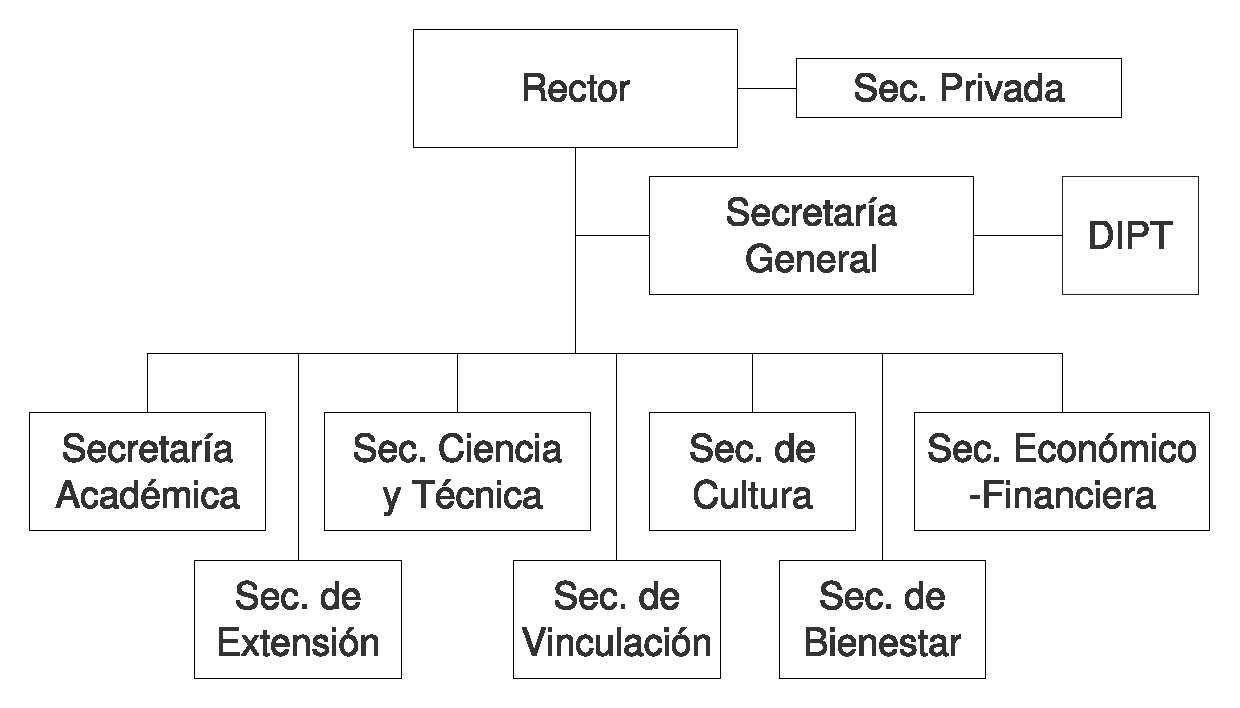
\includegraphics[width=\textwidth]{img/organi_rectorado}
  \caption{Organigrama del Rectorado}
  \label{organi-rectorado}
\end{figure}

Como se puede observar en la figura \ref{mapa-ubicación}, el rectorado
está ubicado en la calle Bv. Pellegrini entre las calles 9 de Julio y
San Jerónimo, en la ciudad de Santa Fe.

\begin{figure}
  \center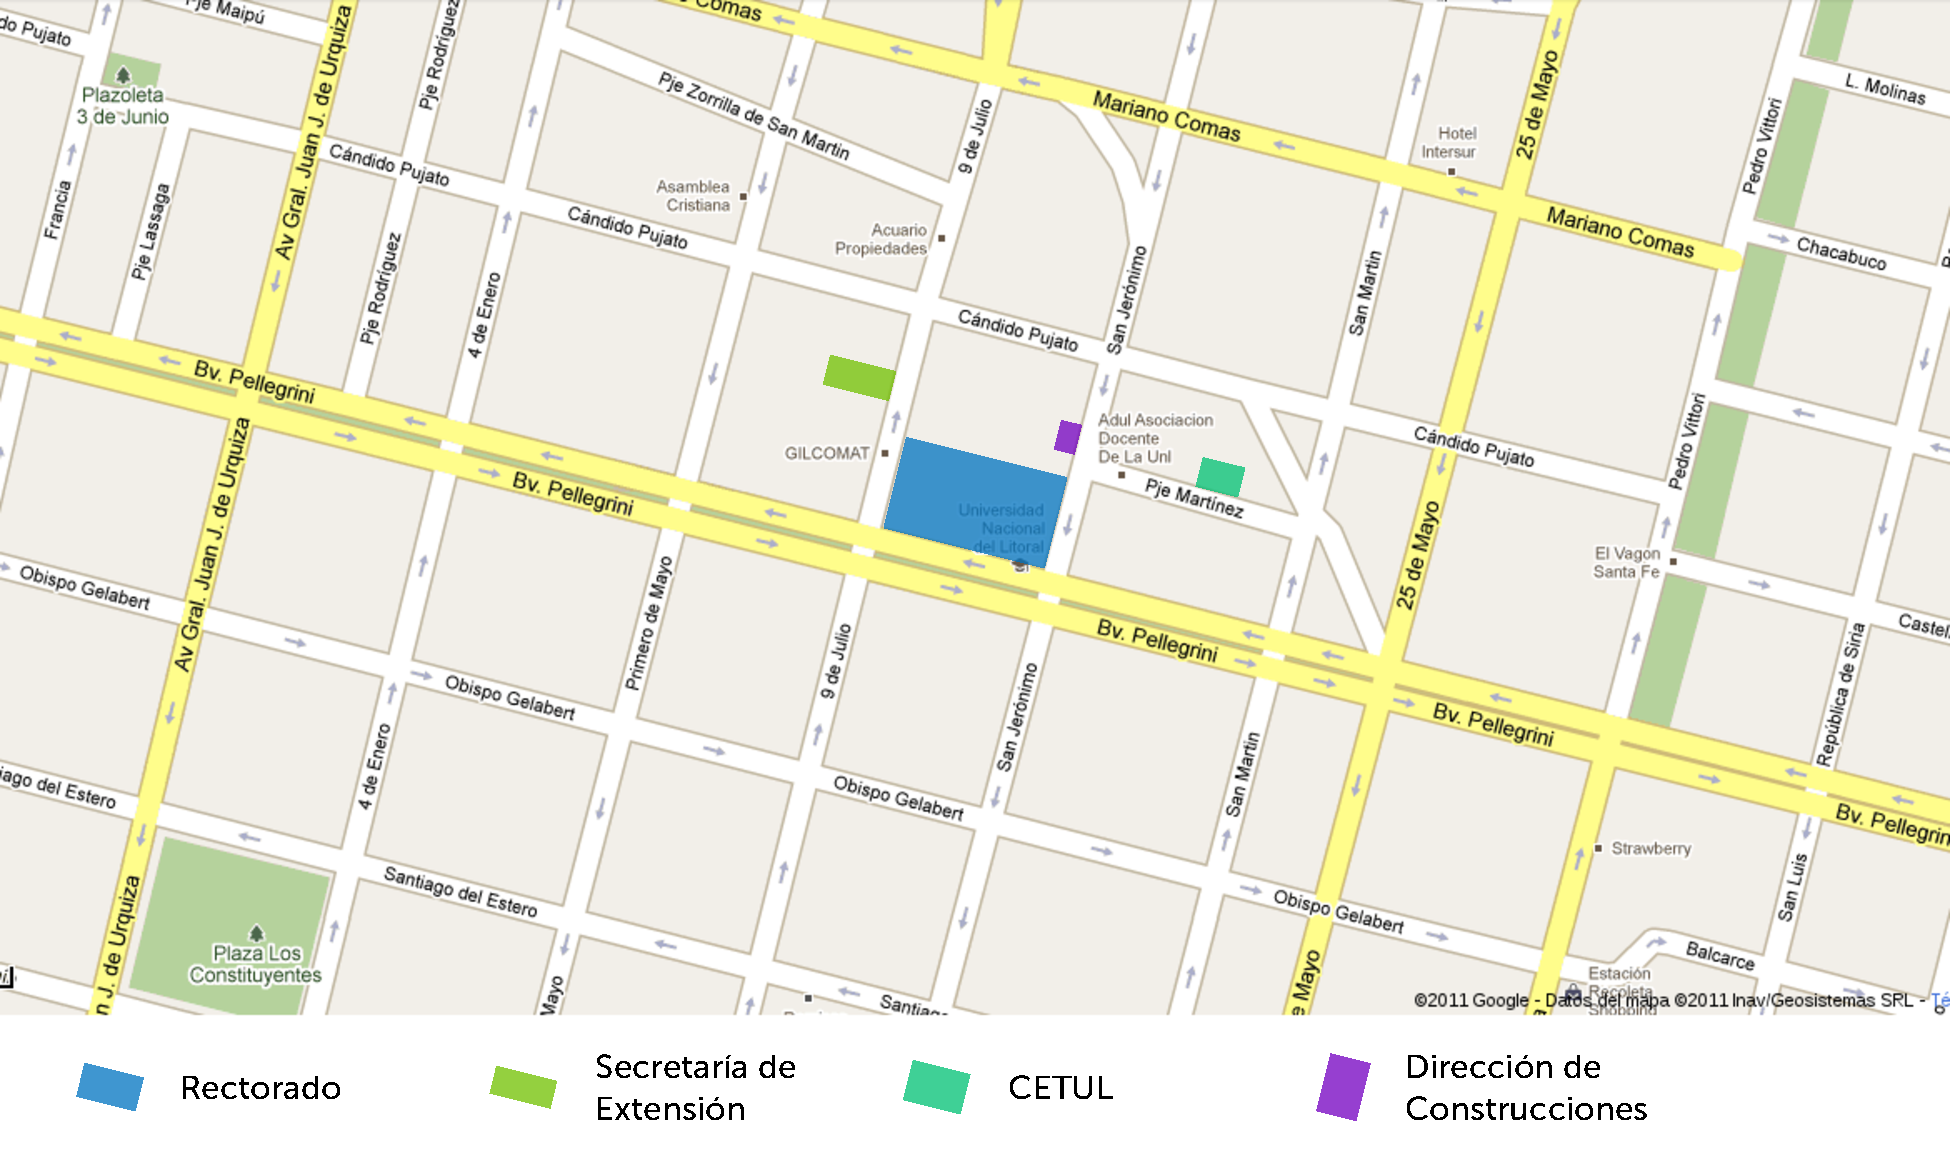
\includegraphics[width=\textwidth]{img/ubicacion_rect}
  \caption{Ubicación del Rectorado en la ciudad de Santa Fe}
  \label{mapa-ubicación}
\end{figure}

%
\section{El área de sistemas de información}
%
El área de sistemas de información es la Dirección de Informatización
y Planificación Tenológica, la cual se encarga de llevar a cabo las
tareas de desarrollo, mantenimiento y administracion de recursos
informáticos, servidores, aplicaciones y soporte técnico a los
usuarios finales dentro del rectorado.
Jerárquicamente, esta dirección depende de la Secretaría General.
%
\subsection{Estructura}
%
La DIPT cuenta con unos 30 empleados, y se subdivide en los siguientes
áreas, como se muestra en la figura \ref{organi-dipt}:
\begin{description}
\item[Cómputos]
  Se encarga del desarrollo, mantenimiento y soporte técnico del
  sistema de gestión de personal SIU Pampa y de la impresión de los
  recibos de sueldo.
%
\item[Desarrollo]
  Su función principal se basa en el desarrollo e implementación de
  sistemas propios y la implementación de los sistemas desarrollados
  por SIU, como el de gestión contable SIU Pilagá, el de gestión de
  alumnos SIU Guaraní, etc. Además se encarga del mantenimiento y el
  soporte técnico a los usuarios de estos sistemas.
%
\item[Administración de Sistemas]
  Se ocupa de la implementación y del correcto funcionamiento de los
  servidores (correo, web, sistemas, etc), la planificación de la
  infraestructura de la red y la compra de equipamiento de red y
  servidores.
%
\item[Seguridad de Sistemas]
  Se encarga de la inspección y revisión de la seguridad de los
  sistemas y redes.
%
\item[Soporte técnico]
  Este sector provee asistencia técnica a los usuarios en sus puestos
  de trabajo.
\end{description}
%
\begin{figure}[H]
  \center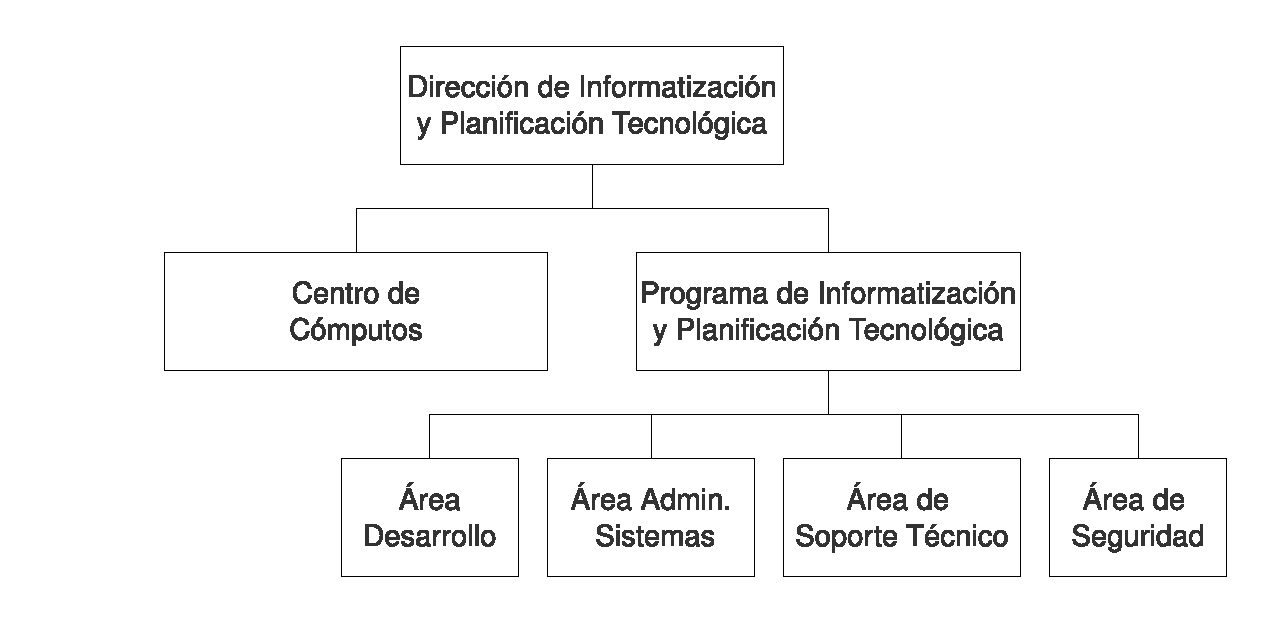
\includegraphics[width=127mm]{img/organi_dipt}
  \caption{Organigrama de la DIPT}
  \label{organi-dipt}
\end{figure}
%
\section{Estrategias informáticas a corto, mediano y largo plazo}
%
La planificacion de las estrategias infomáticas se da mayormente en la
parte de administración junto con el director de la Dirección.

Entre las estrategias a corto plazo podemos citar:
%
\begin{description}
%
\item[Estandarización de los equipos GNU/Linux:]
  %% Actualmente los equipos con GNU/Linux presentan poca uniformidad en
  %% la configuración, y falta de mantenimiento, lo que en la práctica
  %% dificulta el soporte técnico a los usuarios y la administración
  %% remota.  Por esto se hace necesario lo tanto es necesario
  %% reinstalarlas con una versión de Debian estable y una configuración
  %% normalizada.
  Se pretende normalizar las configuraciones y versiones de los
  sistemas en las máquinas con GNU/Linux, ya que éstas presentan
  sistemas en diferentes versiones y estados de configuración, lo que
  dificulta el mantenimiento de estos sistemas.
  %% El sistema operativo Debian ha publicado una nueva versión estable
  %% del mismo. Esta actualización provocó que la gran mayoría de los
  %% equipos con GNU/Linux quedaran en un estado intermedio entre la
  %% versión anterior y la actual, volviéndolos inmantenibles. Se hace
  %% necesario entonces llevar los equipos a la nueva versión estable.
  %% La configuración normalizada se logra mediante la utilización de
  %% scripts desarrollados por personal de soporte técnico y disponible
  %% en un repositorio SVN, que se ejecutan luego de la instalación del
  %% sistema estándar.  Esta tarea se está llevando a cabo lentamente
  %% debido a la falta de personal.
%
\item[Actualización de los servidores a la nueva versión estable de
  Debian:]
  Al igual que ocurrie con las máquinas de los usuarios,
  %% Dado que se ha publicado una nueva versión del sistema operativo
  %% GNU/Linux,
  se hace necesario actualizar el sistema en estos y ajustar las
  configuraciones a las nuevas versiones de los programas.
%
\item[Migración y actualización del servidor de correo:]
  Consiste en la instalación de un nuevo servidor de correo
  electrónico y su interfaz de webmail, realizando el traspaso de
  datos desde el servidor actual al nuevo.
%
\item[Sistema de gestión para el Programa Padrinos:]
  Se trata de desarrollar e implementar el software de facturación e
  impresión de recibos para el Programa Padrinos UNL, perteneciente a
  la Secretaría de Vinculación tecnológica y Desarrollo Productivo,
  dado que el sistema actual se encuentra obsoleto y con problemas
  graves de usabilidad. Esta estrategia se encuadra dentro de la
  implementación del sistema Ilitia.
%
\end{description}

Entre las estrategias a mediano plazo podemos citar:
%
\begin{description}
\item[Migración a software libre:]
  Con el desarrollo de esta estrategia se pretende que todos los
  equipos de la red, tanto clientes como servidores, ejecuten sólo
  software libre, basado en GNU/Linux como sistema operativo base.
  Esta estrategia obedece a una resolución del Honorable Consejo
  Superior, que establece la utilización exclusiva de software libre
  en todo el Rectorado de la Universidad y sus dependencias.
%
\item[Capacitación a los usuarios:]
  Al tiempo que se realiza la migración a entornos de software libre
  se torna fundamental brindar capacitación a los usuarios en el uso
  del nuevo sistema operativo y aplicaciones libres.
  %% Un punto fundamental, que requeriría atención inmediata luego de la
  %% migración sería la capacitación de los recursos humanos para
  %% enfrentar el cambio de sistema operativo y aplicaciones libres.
%
\item[Sistema Ilitia:]
  Se trata del desarrollo y puesta en funcionamiento del sistema, el
  cual sirve para la gestión de los ``Servicios A Terceros Altamente
  Especializados'' y ``Servicios Educativos a Terceros'' (SATs/SETs) y
  demás aspectos de las relaciones Universidad--Empresas.  Dado que el
  consorcio SIU no ofrece un sistema de este tipo, se ha optado por
  desarrollar uno propio.  Actualmente se está comenzando a
  implementar en las distintas áreas de la Secretaría de Vinculación.
%
\item[Adecuación de la sala de servidores:]
  Actualmente la sala de servidores cuenta con un espacio ajustado.
  %% TODO: mover lo que sigue al lugar correspondiente
  %% Hay en existencia dentro de ésta 2 racks que contienen a los
  %% servidores principales, los servidores de almacenamiento RAID y las
  %% unidades de backup en cinta.
  Se está contemplando la posibilidad de expansión, además es
  necesario agregar un segundo aire acondicionado que funcione como
  back-up, piso falso para lograr un cableado ordenado, control de
  acceso mediante llaves o dispositivo de clave, y evitar la
  existencia de elementos no propios de una sala de servidores.
%
\item[Proyecto ``/oficina'':]
  Se trata del desarrollo e implementación de un proyecto tipo CMS
  (\eng{Content Management System}) para brindar a las distintas
  oficinas del rectorado su propio espacio web tanto en la intranet
  como en internet, mejorando la administración, compartición y
  publicación de archivos y documentos.
%
\item [Guía de trámites online para los usuarios:]
  Contempla el poner a disposición de los usuarios los formularios
  para realizar los trámites que se manejan en la oficina de
  informática, por ejemplo: solicitud de habilitación de nodo,
  creación de cuentas de correos, gestión de alias.
\end{description}

Entre las estrategias a largo plazo podemos citar:
%
\begin{description}
\item[Seguridad:]
  Evitar la utilización de software ilegal, encontrar y
  erradicar virus y programas maliciosos, definición de procedimientos
  para protección de los datos, control de acceso a los recursos,
  utilización de sistemas de validación y encriptado para los
  sistemas que manejan información sensible, securización de los
  servidores de correo mediante autenticación y encriptación,
  implementación de sistemas de detección de intrusos.
%
\item[Puppet:]
  Se trata de implementar un sistema de control centralizado de la
  configuración de los equipos. Luego de una implementación fallida y
  posterior caída en desuso, se pretende que el equipo de
  administración y soporte técnico se capacite con este sistema y lo
  ponga en funcionamiento para así gestionar la configuración de los
  equipos de manera centralizada y prácticamente automática,
  resultando en una simplificación del trabajo del personal.
\end{description}
%
\newpage\section{Hardware}
%
El inventario del hardware de Rectorado es llevado por la
Dirección de Patrimonio, externa a la DIPT.

A continuación, se presenta un resumen del hardware disponible en la
DIPT, y el resto de los pisos 3 y 2 del rectorado a modo de ejemplificación.
%
\begin{description}
  \item[Piso 3]: En este piso encontramos la DIPT y la oficina de Personal y Haberes.
  %
    \begin{description}
      \item[DIPT]:
      %
      \begin{itemize*}
      \item 27 workstations
      \item 2 notebooks
      \item 2 impresoras
      \item 1 multifunción
      \item 5 teléfonos
      \item 5 aires acondicionados
      \item 1 cañón
      \item 3 switches
      \end{itemize*}
      %
      A su vez dentro de la DIPT encontramos la sala de servidores que cuenta con:
      \begin{itemize*}
      \item 8 servidores generales
      \item 2 servidores de almacenamiento RAID
      \item 1 PC clon (Firewall)
      \item 2 switches raíz
      \item 1 aire acondicionado
      \item 2 racks con servidores
      \item 2 UPS, uno en cada rack
      \end{itemize*}
      %
      \item[Personal y Haberes]:
      \begin{itemize*}
      \item 20 workstations
      \item 6 impresoras
      \item 1 multifución
      \item 9 teléfonos
      \item 2 aires acondicionados
      \item 2 switches
      \end{itemize*}
    \end{description}
    %
  \item[Piso 2]: En este piso se encuentra la Dirección General de Administración,
    y la oficina de Despacho General y Consejo Superior.
  %
    \begin{description}
      \item[DGA]:
      \begin{itemize*}
      \item 26 workstations
      \item 18 impresoras
      \item 1 multifunción
      \item 16 teléfonos
      \item 3 aires acondicionados
      \item 3 switches
      \item 2 fax
      \item 1 fotocopiadora
      \end{itemize*}
      \newpage
      \item[Despacho General, Consejo Superior]:
      \begin{itemize*}
      \item 10 workstations
      \item 4 impresoras
      \item 4 teléfonos
      \item 1 aire acondicionado
      \item 1 switch
      \item 1 fax
      \end{itemize*}
    \end{description}
\end{description}
%
\section{Software}
%
\subsection{Software base}
%
\subsubsection*{Sistema operativo}
Tanto en el Rectorado como en la DIPT, se utiliza principalmente el
sistema operativo Debian GNU/Linux y en menor medida Microsoft Windows
XP y 7. En las notebooks personales de los usuarios también podemos
encontrar Microsoft Windows Vista, así como Ubuntu y Kubuntu
GNU/Linux.
%
\subsubsection*{Antivirus}
El Centro de Telemática de la UNL (CETUL) ha adquirido licencias para
la utilización del antivirus Sophos AV, sin embargo, éste es poco
amigable y no muy robusto. El más utilizado es el Avira Antivir Free,
que es el que instala el personal de soporte técnico en las máquinas
de los usuarios. También encontramos el AVG Free Edition y el Nod 32,
entre otros.
%
\subsubsection*{Base de datos}
%
Tanto en los sistemas desarrollados internamente como en los del SIU
se utiliza PostgresSQL como motor de base de datos principal. En
algunos sistemas heredados se utiliza además MySQL y MS Fox.  Los
servidores de base de datos son mantenidos por el área de
Administración, mientras que las bases en sí son mantenidas por los
desarrolladores de los distintos sistemas (áreas Desarrollo y
Cómputos).
%
\subsection*{Software aplicativo}
%
\subsubsection*{Software de programación}
%
Para el desarrollo de los sistemas propios se utiliza principalmente
el lenguaje Java, y el software de SIU está desarrollado
principalmente en PHP. También encontramos sistemas en ASP.

Las IDEs que se utilizan son Netbeans, Eclipse y GNU Emacs.

Se utiliza el sistema de versionado de código SVN, mantenido por los
administradores en un respositorio centralizado en los servidores
propios.
%
\section{Esquema de telecomunicaciones}

En la sala de servidores encontramos 8 servidores rackeados en 2
racks, y un tercer rack más pequeño que contiene los 2 switches
raíz. También encontramos el firewall que es simplemente un PC clon
con 4 interfaces de red Gigabit.

La red está implementada mediante 4 redes virtuales (VLANs) manejadas por
los switches raíz. Estas diferentes VLANs son:
\begin{enumerate}
\item Internet (red externa)
\item Intranet (red interna)
\item DMZ1 (zona demilitarizada 1)
\item DMZ2 (zona demilitarizada 2)
\end{enumerate}

El firewall es el dispositivo encargado de regular los accesos entre
las diferentes redes, permitiendo sólo aquellos accesos autorizados, y
evitando la posibilidad de determinados ``ataques'' conocidos a las
redes.

La conexión a la red externa es provista por el Centro de Telemática
de la UNL, físicamente se trata de un enlace de fibra óptica que llega
a uno de los switches raíz y a través de éste conecta directamente al
Firewall.

La red interna es la red donde se ubican las estaciones de trabajo de
los usuarios.  A uno de los switches raíz se conectan mediante fibra
óptica 8 switches centrales que sirven a los niveles inferiores del
rectorado, a saber: uno en el segundo piso, tres en el primer piso,
dos en planta baja, uno en la Dirección de Construcciones (sobre calle
San Gerónimo) y por último uno en la Secretaría de Extensión
Universitaria, sobre calle 9 de julio. En el tercer piso encontramos 4
switches conectados a este switch raíz: 3 en la DIPT y uno en la
Dirección de Personal y Haberes.

Al otro switch raíz se conectan los 8 servidores de la sala de
servidores.  De estos servidores, los 8 están conectados a la
intranet, 4 de ellos están conectados además a la DMZ1 y a la DMZ2, y
2 están conectados a la DMZ1 únicamente.

Estos 8 servidores en realidad implementan como máquinas virtuales
diferentes los servicios como el correo electrónico, bases de datos,
sistemas internos y esternos, etcétera.

La razón de ser de las zonas demilitarizadas es que son partes de la
red a la que sólo están conectados determinados servidores
(virtuales), y para acceder a estos servicios es necesario atravesar
el firewall, permitiendo así un mayor grado de seguridad y un mayor
control acerca de qué accesos están autorizados y cuáles no. Por
ejemplo, el servidor de correo electrónico es una máquina virtual que
tiene una única interface de red, conectada a la DMZ1. Así,cuando un
usuario desea acceder al servidor, deberá necesariamente atravesar el
firewall para ello. Además, si se tratara de un usuario malicioso y
éste lograra comprometer el servidor de correo, el hecho de que tiene
que atravesar el firewall para alcanzar otros servidores y/o las
máquinas de los usuarios limita su capacidad de potencial daño.

Por último, encontramos que los 8 servidores poseen otra interface de
red, que están conectadas a un switch aislado. Esta red es exclusiva
para sincronización de datos entre los servidores. No está conectada a
ninguna otra red y sirve sólo a las funcionalidades de los servidores.

En la figura \ref{topologia} vemos gráficamente el esquema de la red
de teleprocesamiento aquí descrita.
%
\begin{figure}[h]
  \center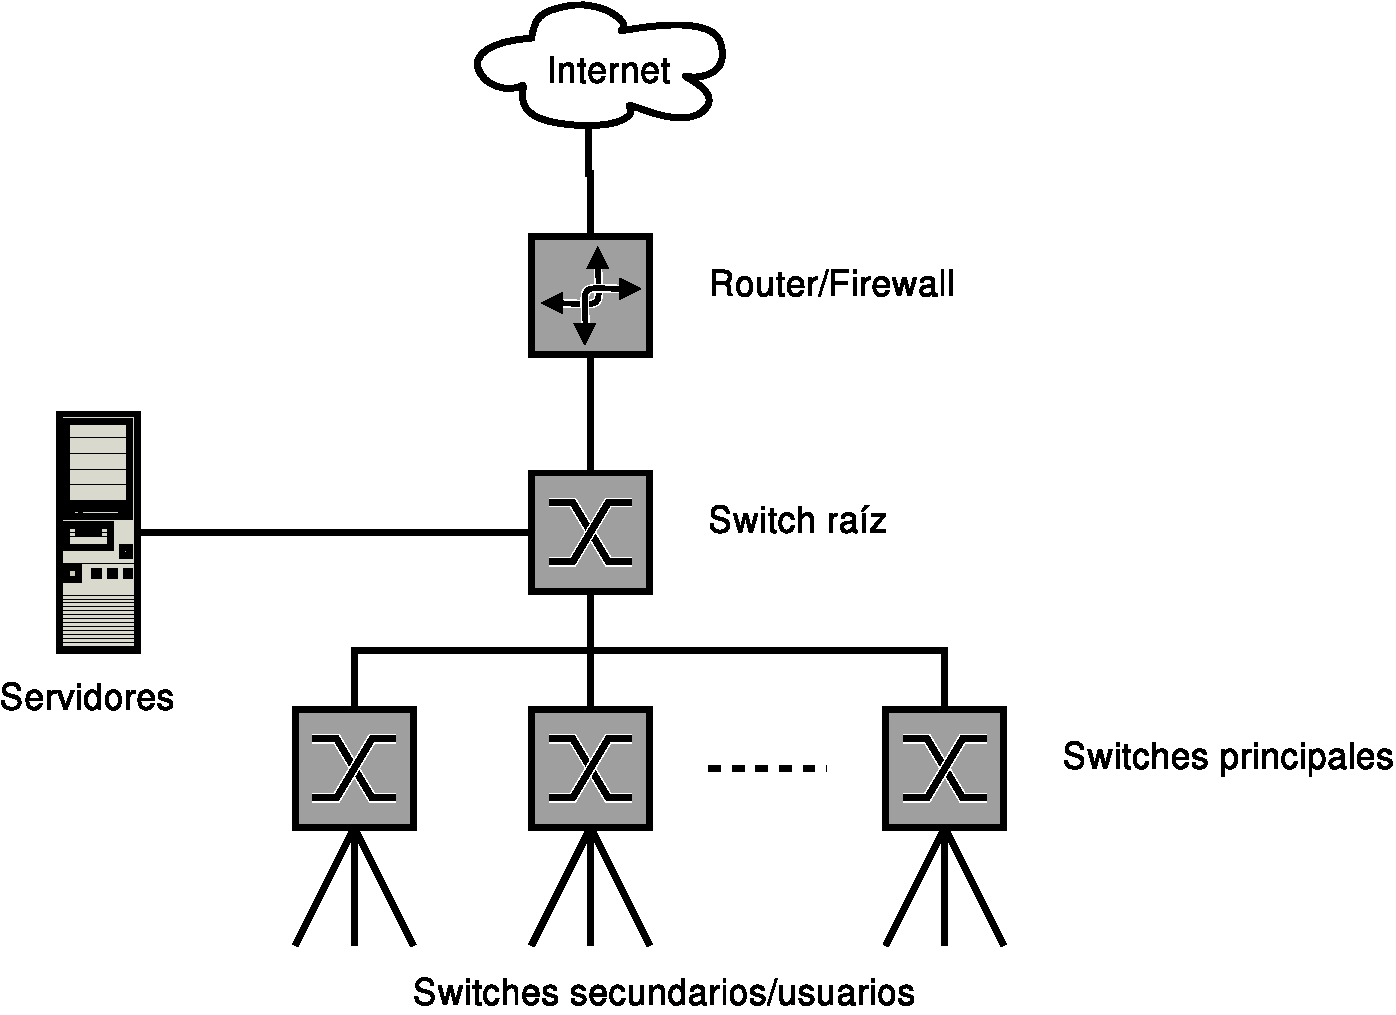
\includegraphics[width=\textwidth]{img/red}
  \caption{Esquema de la topología de la red en el Rectorado.}
  \label{topologia}
\end{figure}
%
\newpage
\section{Normativa interna}
%
Existen determinadas normativas respecto del uso de la red, impuestas
por el Centro de Telemática (CETUL), que es el órgano encargado del
manejo e interconexión desde la Universidad a Internet y otras redes
externas, y provee de conexión a las diferentes instituciones de la
UNL.

Los usuarios deben firmar un acuerdo de conformidad tanto al solicitar
la creación de una cuenta de correo electrónico perteneciente al
rectorado, como al requerir la habilitación de una nueva computadora
en la red interna.

Algunos de los puntos de este acuerdo de conformidad establecen lo
siguiente:
%
\begin{itemize*}
\item Prohibición de utilizar los servicios de la red para uso
  comercial particular,
\item prohibición del uso de la red con fines de hackeo/cracking, y
  difusión de virus/spy\-ware/malware, y
\item prohibición de la utilización de la cuenta de correo electrónico
  para envío de spam.
\end{itemize*}
%
\subsection*{Procedimientos internos de la DIPT}
%
\begin{description}
\item[Atención a usuarios:] el siguiente esquema se sigue para brindar
  soporte técnico a los usuarios:
  \begin{enumerate*}
  \item Los usuarios inician una solicitud llamando
    a un número telefónico dispuesto a tal efecto.
  \item Se asigna a la petición un número de caso completando un
    ``ticket'' en un sistema de seguimiento.
  \item El técnico se encarga de revisar la lista de tareas
    pendientes, asignándose un caso de la lista para atender,
    realizando un seguimiento del progreso en el sistema.
  \item Una vez resuelto el problema, se cierra el caso en el sistema.
  \end{enumerate*}
\item[Tickets:] el sistema de tickets es utilizado por casi todos los
  sectores del área, siendo éste la forma de comunicación más
  común entre los distintos sectores del área de Informática.
\item[Software libre:] salvo casos excepcionales, la política de
  rectorado establece que sólo se utilizará software libre en las
  estaciones de trabajo y en los servidores.
\item[Software del SIU:] la UNL adhiere al consorcio SIU, lo que
  implica que la mayoría de los sistemas de la Universidad provienen
  del mismo.
\end{description}
%
\newpage
\section{Relaciones con terceros}
La DIPT provee servicios de administración, mantenimiento y soporte
técnico de sistemas a diversas áreas de la Universidad.

Además de esto, en la Dirección se manejan relaciones principalmente
con proveedores de hardware, insumos y servicios informáticos.

Las compras de equipamiento se realizan según la normativa establecida
por el Rectorado.  Ésta establece que las compras menores a \$2400 se
pueden efectuar directamente, mientras que para aquellas que superan
este monto es necesario pedir tres presupuestos a diferentes empresas.
Una vez obtenidos estos presupuestos se debe iniciar un expediente a
través de Mesa de Entrada, en el cualse deben incluir éstos junto a un
cuadro comparativo donde se justifique la adjudicación de la
compra. Además, si la compra supera los \$10000, se deberá llamar a
licitación con una solicitud a la Dirección de Compras y
Contrataciones.
%
\section{Politicas de selección, capacitación y entrenamiento de personal}
%
No existen políticas específicas para la selección del personal, más
que un simple criterio basado en la idoneidad para el puesto y
experiencia de trabajo previa, entre otros.

El personal de la Dirección realiza ocasionalmente cursos de
capacitación relacionados con la actividad en la que trabajan día a
día.

Las áreas de Desarrollo y de Cómputos asisten a los encuentros
realizadas por el SIU relacionados con la implementación de sus
sistemas.

El área de Administración de Sistemas realiza dos veces al año pruebas
de stress en determinados sistemas, y también simulaciones con
sistemas experimentales para el entrenamiento y ``sincronización de
conocimientos'' entre sus miembros.

Además, tanto las áreas de Desarrollo y de Administración de sistemas
realizan encuentros semanales en donde se discuten los temas donde se
hace necesaria una capacitación en profundidad de alguno de los
integrantes.

El área de seguridad realiza charlas al respecto, en general
orientadas al área de Administración de Sistemas.

En casos excepcionales determinadas personas asisten a cursos de
capacitación/seminarios específicos dictados en general en Buenos
Aires.
%
\newpage
\section{Problemas, necesidades e incertidumbres existentes en la organización}
%
\subsection*{Redundancia de los enlaces de red}
En ninguna parte de la topología de la red encontramos enlaces
redundantes. Esto resulta en un riesgo alto de dejar fuera de servicio
a sectores del Rectorado en caso de falla de una interface de red en
los servidores o en una boca de un switch central. También genera un
riesgo en caso de corte de los cables de cobre y ópticos,
especialmente los enlaces de fibra más extensos como los que sirven a
la Secretaría de Extensión y a la Dirección de Construcciones
Universitarias.

Sin embargo, encontramos que existen cables de cobre UTP que han
quedado instalados hacia varios de los switches centrales luego del
traspaso a conexiones de fibra óptica, aunque éstos se encuentran
desconectados y en desuso.
%
\subsection*{Sala de servidores}
El espacio de la sala de servidores es el adecuado para la cantidad de
equipos que hay actualmente, sin embargo, si en un futuro se quisiera
agregar otro rack para ampliar la capacidad operativa, no sería
posible dado que el espacio sería insuficiente.

Un problema que presenta la sala es que una falla en el acondicionador
de aire podría traer problemas serios, dado que no existe un
acondicionador de ``back-up'' en caso ue falle el principal. Este
riesgo es particularmente alto en el verano, cuando el aire
acondicionado funciona en toda su capacidad.
%
\subsection*{El espacio de trabajo del personal es reducido}
El sector de informática con el paso del tiempo a incrementado el
número de los puestos de trabajo. Pero el espacio de trabajo sigue
siendo el mismo, por lo tanto el espacio físico no es suficiente. El
mismo tiene 5[m] por 10[m] de dimensión y trabajan en este espacio 25
personas.
%
\subsection*{No existe un plan de contingencia ante fallas eléctricas}
Actualmente no existe un plan de contingencia ante eventuales fallas
en el suministro eléctrico. La oficina cuenta con un UPS centralizado
que permite mantener el suministro eléctrico en las PCs de los
usuarios y los servidores durante unos 10 minutos. Es bastante común
que ocurran fallas en los servidores luego de restablecido el
suministro, porque el tiempo que brinda el UPS no alcanza para que los
servidores terminen de realizar sus tareas de apagado de forma óptima.
%
\subsection*{No existe control de acceso físico}
El acceso físico de las personas al lugar no está controlado,
existiendo la posibilidad de que ingrese alguna persona
malintencionada y ocurra por ejemplo robo de equipamiento. Esta
posibilidad aumenta durante la tarde, cuando hay pocas personas
trabajando en el lugar.

El área no posee cámaras de seguridad o algún bloqueo del tipo físico,
como llaves o dispositivos de autorización por tarjeta/llave o
similar, por lo tanto consideramos que existen falencias de seguridad.
%
\subsection*{Seguridad Lógica}
En todo el Rectorado la red a la que se conectan las estaciones de
trabajo es cableada (Ethernet), no hay servicio de Wi-Fi provisto por
la DIPT. Para el acceso a la red física, el usuario debe solicitar la
habilitación de su PC en la red mediante el llenado de un formulario.

Esta autorización resulta en el agregado de la PC a la lista de
equipos autorizados, otorgándole una entrada en el servidor DNS y el
DHCP. Este servidor DHCP es el encargado de asignarle una dirección IP
a la máquina del usuario cuando éste la conecta a la intranet.

Sin embargo, un sujeto malintencionado puede conectar directamente una
PC y asignarle una dirección IP manualmente sin pedir
autorización. Esto es posible dado que no existe ningún tipo de filtro
de MAC o algún protocolo de autenticación mediante certificados o
firmas digitales que controle quién accede a la red.

La DIPT provee un servidor de directorio \eng{LDAP} que se utiliza
para autenticar las cuentas de los usuarios al iniciar sesión. Este
mecanismo de autenticación se realiza en muchos casos (sino en la
mayoría) en forma no encriptada, lo que implica que alguien con
conocimientos básicos de técnicas conocidas como ``sniffing'' puede
capturar las claves de los usuarios.

El servicio de correo electrónico que se ofrece utiliza un servidor de
salida SMTP no autenticado, con la única restricción de que el equipo
que se conecta para enviar correos esté dentro de la red interna. Han
ocurrido casos en que computadoras infectadas por ``botnets'' han
enviado masivamente correos electrónicos con spam.

Otro problema de falta de seguridad lo encontramos en la forma en que
los usuarios de Windows comparten sus archivos. En muchos casos, se da
que lo hacen sin protegerlos con contraseña, lo que hace que
cualquiera con acceso a la red pueda tomar el control de sus archivos.

En definitiva, cualquier persona con conocimientos suficientes que
consiga enchufar su PC a la red local, tiene una capacidad
potencial de provocar daños a los sistemas, principalmente en las PCs
de los usuarios.
%
\subsection*{Proyectos abortados}
Es bastante común encontrarnos con que los proyectos se ``congelan'' y
se terminan abortando, lo que puede estar indicando una falta de
coordinación y de tiempo entre las diversas áreas involucradas.

Estos proyectos abortados los encontramos principalmente en las áreas
de administración y de soporte técnico a los usuarios. Los encargados
de estas áreas nos indican que se debe a la saturación de trabajo
``corriente'', o del día a día, lo que hace que no quede tiempo para
la planificación, investigación y capacitación necesaria para
llevarlos adelante.

Varios de los proyectos que forman parte de las estrategias antes
citadas se encuentran en estado de virtual congelamiento, o de
funcionamiento a medias.  Entre ellos encontramos:
\begin{description}
\item[Proyecto Puppet]: este proyecto se inició a finales del año
  2008. Como parte del mismo participaban las áreas de administración
  de sistemas y de soporte técnico.  Se avanzó en el proyecto durante
  el año siguiente según estaba previsto, pero luego a partir de la
  reducción del personal de soporte técnico y la renovación casi
  simultánea del plantel de administración, el proyecto en su conjunto
  ha quedado estancado.
\item[Servidor de correo]: la actualización del servidor de correo
  también se encuentra congelada dado que el proyecto requiere que el
  personal de soporte técnico actualice la configuración de cada una
  de las máquinas de los usuarios. Como el correo electrónico es
  un servicio esencial para el trabajo del personal, esta
  actualización debe realizarse en un tiempo corto, lo cual resulta
  imposible dados los recursos disponibles hoy día.
\item[Capacitación a los usuarios]: estas tareas de capacitación se
  habían planificado como un trabajo extra del personal, coordinado
  por la Secretaría de Coordinación del Rectorado.  Dada la escasez de
  asignación de recursos a las mismas, hoy en día no se están
  llevando adelante.
\item[Proyecto /oficina]: si bien no podemos considerar a este
  proyecto como abandonado, sólo se avanzó en una primera etapa de
  implementación del mismo, y actualmente éste sirve a unas 3
  oficinas. En este caso podemos considerar la falta de coordinación
  entre las áreas de seguridad y administración de sistemas como el
  origen del problema.
\end{description}
%
\subsection*{Falta de mantenimiento en las PCs de los usuarios}
Este es un problema que se ha puesto en evidencia a partir de la
publicación de la nueva versión estable del sistema operativo Debian
GNU/Linux, usado en la mayoría de las estaciones de trabajo en febrero
de este año.

Una falta de mantenimiento de la configuración por parte del equipo de
soporte técnico y de administración provocó que sin haberlo previsto,
los equipos de los usuarios se actualizaran automáticamente, fallando
en medio del proceso, lo que los volvió inusables por parte de los
usuarios.

Entre las causas encontramos además el abandono del proyecto Puppet
iniciado dos años atrás.
%
%% \subsection*{}
%% Así también ocurre que en la implementación de los sistemas, sean
%% tanto desarrollos propios como aquellos provistos por el SIU, existe
%% falta de previsibilidad en cuanto a su rendimiento para el hardware
%% disponible. Además, a los usuarios de estos sistemas se les brinda
%% escasa capacitación respecto del funcionamiento de los mismos.
%
\subsection*{Relaciones comerciales}
Por último, hemos detectado que en la parte administración existe una
única persona encargada de manejar todas las relaciones comerciales
con los proveedores, lo que significa que no existe un control de
éstas por parte del jefe de la dirección, y que cuando esta persona se
ausenta se complican cosas tan corrientes como encargar la recarga de
un tóner.
\newpage
\section{Plan de Mejoras}
\subsection*{Redundancia de los enlaces de red}
Recomendamos agregar enlaces redundantes a la red de área local, al
menos en enlaces principales. A este efecto se deberá considerar la
posibilidad de utilizar los enlaces de cobre preexistentes a la fibra,
para lo cual habrá que verificar el estado de estos cables. En caso de
que no estén en condiciones, habrá que evaluar si conviene
reemplazarlos por cables nuevos o configurar enlaces
inalámbricos. Sería conveniente analizar la posibilidad de colocar
enlaces de fibra que permitirán soportar eventuales amplicaciones de
la capacidad de la red.

También es de vital importancia dotar de redundancia a los enlaces y
switches de la sala de servidores, esto además traerá la ventaja del
aumento de velocidad de los mismos.
%
\subsection*{Sala de servidores}
Se deberá considerar la expansión de la sala de servidores. Para esto
se deberán evaluar tres posiblidades, una de ellas es reubicar el área
de soporte técnico en otra oficina dentro del mismo rectorado y así
ocupar el espacio que ocupa actualmente para la ampliación de la sala.
Otra posibilidad es realizar una reforma edilicia que involucre
reubicar los puestos de trabajo y la sala de servidores dentro del
mismo espacio físico, logrando así un mejor aprovechamiento del lugar.
Como úlima opcion proponemos la posibilidad de mudar la sala de
servidores a otro sector del rectorado o incluso a otro edificio, como
puede ser la Secretaría de Extensión Universitaria.

También se hace imperativo instalar otro equpo de aire acondicionado,
para salvaguarda del existente en caso de alguna falla.
%
\subsection*{El espacio de trabajo del personal es reducido}
Dado que la oficina DIPT cuenta con tres áreas: administracion y
desarrollo, soporte técnico y cómputos, se podría replantear la
ubicación de los recursos humanos de cada área. Dado que el personal
de administración y desarrollo es mas numeroso, proponemos reubicar a
los empleados de soporte técnico y de cómputos hacia otras oficinas y
así mejorar el espacio de trabajo en la oficina actual.
%
\subsection*{No existen un plan de contingencia ante fallas eléctricas}
Se deberá elaborar un plan de contingencia, así como terminar de
colocar el grupo electrógeno adquirido recientemente.  También sería
conveniente modificar la instalación eléctrica de la oficina,
separando los tomas para el qeuipamiento informático de aquellos de
uso general.
%
\subsection*{No existe control de acceso físico}
Es conveniente colocar cámaras de seguridad para monitorear el espacio
de trabajo de la oficina. Pero para controlar el acceso a la sala de
servidores, es conveniente tener mayor seguridad. Esto se lograría
colocando llave o un control de acceso mediante un sistema de
detección de huellas digitales.
%
\subsection*{Seguridad lógica}
Se deberá investigar la factibilidad de incorporar tecnología de
autenticación mediante un servidor RADIUS a la red de área local.
Esta no será una tarea menor, ya que se hace necesario configurar todos
los equipos de la red, desde servidores hasta las impresoras en red, incluyendo
las PCs de los puestos de trabajo y los switches.

Lo más conveniente sería entonces diseñar un plan de implementación
gradual, como puede ser el siguiente:
\begin{enumerate}
\item Comenzar por incorporar esta tecnología de autenticación a
  aquellos servicios que manejan información crítica, y aquellos
  puestos que trabajan con estos sistemas.
\item Seguir por los sistemas y puestos de trabajo que manejan
  información confidencial pero no crítica.
\item Finalmente, incorporar al resto de los usuarios y el
  equipamiento como impresoras de red, lo cual traería consigo el
  beneficio de que todos los usuarios podrán estar seguros que el
  entorno de red al que se conectan es fiable y controlado.
\end{enumerate}

En lo que refiere al servidor LDAP, es imperativo volver a configurar
la utilización del servicio a través de HTTP seguro (HTTPS) para
evitar que las contraseñas de los usuarios estén viajando en texto
plano a través de la red.

En lo que refiere al servidor de correo electrónico, se hace necesario:
\begin{itemize*}
\item Incorporar autenticación al servidor de salida SMTP, y
  establecer una cuota máxima de correos permitidos por usuario por
  unidad de tiempo (por ejemplo, que un mismo usuario no pueda enviar
  correo a más de 100 personas en un lapso de una hora).
\item Inhabilitar las conexiones no seguras (sin seguridad TLS) tanto
  para el sevidor de salida SMTP, como para los servidores de
  recepción POP e IMAP.
\item Incorporar al cliente de webmail un desafío estilo CAPTCHA, que
  verifique la ``humanidad'' del usuario antes de permitir el envío de
  correo.
\end{itemize*}

Se hace muy conveniente implementar un sistema centralizado de manejo
de documentos, que permita a los usuarios almacenar sus documentos y
compartirlos con otros usuarios. Este sistema debería proveer además
un servicio de backup, e idealmente, un sistema de control de
versiones.

Una vez puesto en funcionamiento el sistema se deberán realizar
capacitaciones a los puestos de trabajo, persuadiéndolos de las
ventajas de utilizar este sistema en lugar de utilizar el servicio
(inseguro) de carpetas compartidas de Windows.

\subsection*{Proyectos abortados}
Proponemos implementar un sistema de seguimiento de proyectos, el cual
debe reunir las siguientes características:
\begin{itemize*}
\item Un plan de tareas de cada proyecto con fechas estimadas de
  concreción.
\item Alarmas que den aviso de incumplimiento de tareas.
\end{itemize*}
Se deberá desarrollar un manual de procedimiento para llevar a cabo un
proyecto nuevo, que estipule la forma de proceder a la hora de
encagarlo.

Para el área de administración y soporte técnico se deberá aumentar el
presupuesto para agregar mas gente que se ocupe de las cuestiones del
día a día. De esta forma quedarían liberadas personas para encargarse
de planificar e investigar.

También habrá que volver a hacer un análisis de los proyectos
virtualmente congelados para dicidir si se reinician o conviene
descartarlos.

\begin{description}
\item[Proyecto Puppet :]conviene poner el estado de este proyetco
  sobre la mesa decidir si se termina de implementr o directamente se
  abandona evaluando los resultados obtenidos hasta ahora.
\item[Servidor de Correo:] con la incorporación de personal al área de
  soporte técnico para ocuparse de las tareas de rutina, se podrían
  actualizar las máquinas del personal para finalmente migrar a la
  nueva configuración del servidor.
\item[Proyecto/oficina :]se debería reasignar el proyecto a alguien de
  admnistración que se encargue de mantener y terminar de implementar
  el sistema.
\end{description}

\subsection*{Falta de mantenimiento en las PCs de los usuarios}
Este problema se podría solucionar poniendo en funcionamiento el
proyecto Puppet, ya que éste gestiona de manera automática la
configuracion de las máquinas de los usuarios.  De ser posible esta
opción debería encargarse el personal de soporte técnico.
\subsection*{Relaciones comerciales}
Se hace conveniente establecer un sistema de gestión de los vínculos
comerciales (este puede ser tan sencillo como una planilla de
cálculo), en donde quede registrado el estado de los pedidos, pagos
etc. A este documento tendrían que tener acceso dos o tres personas de
área de administración y el jefe de la oficina.

\section*{Conclusiones}
En este trabajo hemos presentado una auditoría informática de la DIPT
de la UNL. Se han detectado una serie de problemas en los cuales se
hace patente la falta de personal y de espacio físico de la
organización. Hemos propuesto soluciones que a nuestro criterio son
las mas acertadas.

\end{document}

